%%%%%%%%%%%%%%%%%%%%%%%%%%%%%%%%%%%%%%%%%
% Homework Assignment Article
% LaTeX Template
% Version 1.3.1 (ECL) (08/08/17)
%
% This template has been downloaded from:
% Overleaf
%
% Original author:
% Victor Zimmermann (zimmermann@cl.uni-heidelberg.de)
%
% License:
% CC BY-SA 4.0 (https://creativecommons.org/licenses/by-sa/4.0/)
%
%%%%%%%%%%%%%%%%%%%%%%%%%%%%%%%%%%%%%%%%%

%----------------------------------------------------------------------------------------

\documentclass[a4paper]{article} % Uses article class in A4 format

%----------------------------------------------------------------------------------------
%	FORMATTING
%----------------------------------------------------------------------------------------

\addtolength{\hoffset}{-2.25cm}
\addtolength{\textwidth}{4.5cm}
\addtolength{\voffset}{-3.25cm}
\addtolength{\textheight}{5cm}
\setlength{\parskip}{0pt}
\setlength{\parindent}{0in}

%----------------------------------------------------------------------------------------
%	PACKAGES AND OTHER DOCUMENT CONFIGURATIONS
%----------------------------------------------------------------------------------------

\usepackage{blindtext} % Package to generate dummy text
% \usepackage[style=numeric,sorting=none]{biblatex}
\usepackage{charter} % Use the Charter font
\usepackage[utf8]{inputenc} % Use UTF-8 encoding
\usepackage{microtype} % Slightly tweak font spacing for aesthetics

\usepackage[english]{babel} % Language hyphenation and typographical rules

\usepackage{amsthm, amsmath, amssymb} % Mathematical typesetting
\usepackage{float} % Improved interface for floating objects
\usepackage[final, colorlinks = true, 
            linkcolor = black, 
            citecolor = black]{hyperref} % For hyperlinks in the PDF
\usepackage{graphicx, multicol} % Enhanced support for graphics
\usepackage{xcolor} % Driver-independent color extensions
\usepackage{marvosym, wasysym} % More symbols
\usepackage{rotating} % Rotation tools
\usepackage{censor} % Facilities for controlling restricted text
\usepackage{listings, style/lstlisting} % Environment for non-formatted code, !uses style file!
\usepackage{pseudocode} % Environment for specifying algorithms in a natural way
\usepackage{style/avm} % Environment for f-structures, !uses style file!
\usepackage{booktabs} % Enhances quality of tables

\usepackage{tikz-qtree} % Easy tree drawing tool
\tikzset{every tree node/.style={align=center,anchor=north},
         level distance=2cm} % Configuration for q-trees
\usepackage{style/btree} % Configuration for b-trees and b+-trees, !uses style file!

% \usepackage[backend=biber,style=numeric,
            % sorting=nyt]{biblatex} % Complete reimplementation of bibliographic facilities
% \addbibresource{ecl.bib}
\usepackage{csquotes} % Context sensitive quotation facilities

\usepackage[yyyymmdd]{datetime} % Uses YEAR-MONTH-DAY format for dates
\renewcommand{\dateseparator}{-} % Sets dateseparator to '-'

\usepackage{fancyhdr} % Headers and footers
\pagestyle{fancy} % All pages have headers and footers
\fancyhead{}\renewcommand{\headrulewidth}{0pt} % Blank out the default header
\fancyfoot[L]{School of Computing, Macquarie University} % Custom footer text
\fancyfoot[C]{} % Custom footer text
\fancyfoot[R]{\thepage} % Custom footer text

\usepackage{comment}
\newcommand{\note}[1]{\marginpar{\scriptsize \textcolor{red}{#1}}} % Enables comments in red on margin

%----------------------------------------------------------------------------------------

\begin{document}

%----------------------------------------------------------------------------------------
%	TITLE SECTION
%----------------------------------------------------------------------------------------

\title{COMP3100 project report} % Article title
\fancyhead[C]{}
\hrule \medskip % Upper rule
\begin{minipage}{1\textwidth} % Center of title section
\centering 
\large % Title text size
Project report: Stage 1\\ % Assignment title and number
COMP3100 Distributed Systems, S2, 2022\\
\normalsize % Subtitle text size
SID: 46030190, Name: Thien Luu \cite{code}
%%%%\\ % Assignment subtitle
\end{minipage}
\medskip\hrule % Lower rule
\bigskip

%----------------------------------------------------------------------------------------
%	ARTICLE CONTENTS
%----------------------------------------------------------------------------------------

%----------------------------------------------------------------------------------------
%	1 - INTRODUCTION (1/2 PAGE)
%----------------------------------------------------------------------------------------

\section{Introduction}
The project is a university assignment allocated for COMP3100 students to allow them to build and showcase according to the specifications outlined, their understanding of Distributed Systems given a Distributed Systems simulator. There are 2 stages to it, \textbf{Stage 1} - being assessing the working of code in a demo session, and \textbf{Stage 2} - Offline marking on report, project management and code.
\bigskip

The simulator we are given is a server (ds-server) that simulates all tasks, job submissions, and job execution. The task is to create a client (ds-client) to communicate with the server to schedule jobs (client-server model) using the Largest Round Robin (LRR) algorithm.
\bigskip

Our goal here is to learn how a distributed system functions as we build it - establishing a connection (handshake), then for them to communicate with each other, allocate jobs, add job to queue, complete, and schedule jobs using LRR, and then closing the connection. We will have to perform research, apply Java programming knowledge for the build to develop our understanding and create a report using \LaTeX.

%----------------------------------------------------------------------------------------
%	2 - SYSTEM OVERVIEW (1/2 PAGE)
%----------------------------------------------------------------------------------------

\section{System Overview}
\label{sec:section2}
\subsection*{Server-side}
DS-Sim server-side acts as being a simulator housing servers of types. Jobs are processed by these servers once they are scheduled by the client-side. The server accepts messages from the client that asks the server to process jobs on certain servers it requests or requests server information for the client to determine and other statuses or errors. The server is programmed with a default socket to be 'localhost', on port 50000 for multiple clients to establish a connection to it and schedule jobs.

\subsection*{Client-side}
The Client-side of DS-Sim communicates with the server-side to \textit{only} schedule jobs. To schedule jobs it'll first need to be able to communicate with the server and to do this it'll connect to the server-side socket (assuming the server is already running). We then declare two variables to talk. One to send and the other to receive using 'OutputStream' and 'InputStream' respectively. The client is ready to communicate, the client will initialize communication via a handshake sending 'HELO' to the server, the server then responds 'OK'.

\bigskip
Now that they are connected, on the server-side, before being able to schedule jobs, the server is programmed and requires the client to authenticate, which the client sends 'AUTH \textit{name}', the server responds 'OK'. Here the Client sends 'REDY' to indicate they are ready to acquire Job information, request server information, schedule jobs on available servers, and handle any job errors that arise - information received from the server and for the client to handle. These information request processes will be implemented with loops as there are multiple jobs to be scheduled. Once all jobs have completed processing, the client will terminate the connection with the server with 'QUIT' and close the socket.

%----------------------------------------------------------------------------------------
%	3 - DESIGN (1 PAGE)
%----------------------------------------------------------------------------------------
\break
\section{Design}
\label{sec:section3}
DS-Sim is acting as both a server and user, we are creating a client being the middleman to accept jobs from DS-Sim (user) and return jobs to DS-Sim (server) to process. Before scheduling jobs accordingly to the LRR algorithm requirement, we need to determine the right servers to use by requesting server information, see what server types there are, how many there are, and cores.

\medskip
\textit{The design does not implement XML file reading, where the client reads an XML file containing the settings of servers to be created by the server. The client is treated as a remote client not read files remotely via the connection, only able to send and receive messages - to request and submit information}

\begin{figure}[!h]
    \centering
    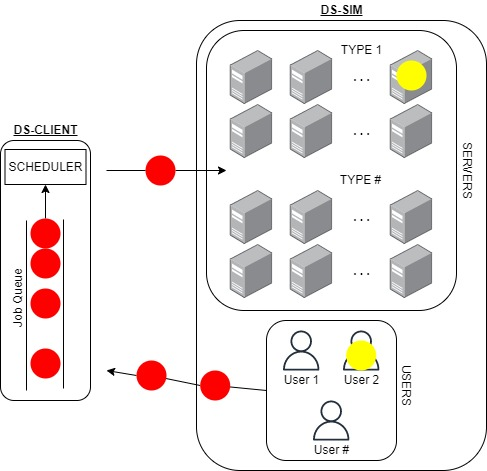
\includegraphics[width=7cm]{images/ds-serverANDclient diagram.jpg}
    \caption{Using DS-Sim}
    \label{fig:my_label}
\end{figure}

\subsection{Communication with DS-Sim}
According to the ds-sim configuration, there are many messages to receive in different stages of communication. Conditional statements will have to be used to simplify the handling of messages. Messages received for example are to perform processes, request information, or errors. Having this sort of handling allows for future expansion if the server side is updated for example with new messages and we can add messages to send and handle.

\medskip
With communication over socket programming, we'll have separate methods, one for sending messages, and one for receiving messages. This will keep the code cleaner, \cite{advantagesofoop} reusable and modular

\subsection{Selecting Server for scheduling}
The requirements are to use the server group of \textit{a type that is the first one to be added}, of the \textit{largest core} to be used for processing jobs. The design will require loops to iterate through the servers information received from the DS-Sim to be sorted and the correct server can then be used.

\subsection{Scheduling Jobs}
Scheduling jobs must be done using the LRR algorithm. To do this, once we have the server group of type, we have a loop, and in the loop, schedule a job to a server and then increment the 'serverid' to be used for the next loop iteration scheduling a job to a different server of the same type. This process cycles until the DS-Sim indicates with a message saying there are no more jobs to schedule. Once the 'serverid' reaches a point where there are no more servers of that type available, the 'serverid' resets and starts scheduling from the first server it scheduled a job on. If a job is still being processed, the new job is still scheduled but it is queued to be processed as soon as the one currently processed finishes.

\subsection{Object}
Jobs and Servers have their attributes according to the specifications, and following best code design practices, we can achieve \cite{advantagesofoop} flexibility and modularity with the use of objects. We'll have a Job and Server class BUT for Stage 1, only Server will be implemented.

%----------------------------------------------------------------------------------------
%	4 - IMPLEMENTATION (2 PAGE)
%----------------------------------------------------------------------------------------
\break
\section{Implementation}
\subsection*{Classes}
\textbf{-=ServerState=- \textit{implements} Comparable}
\begin{flushleft}
    \begin{tabular}{|l|l|l|}
        \hline
        \textbf{Attribute Name} & \textbf{Data Type} & \textbf{Description} \\
        \hline
        Type & String & Type of Server \\
        \hline
        ServerId & Integer & ID of Server\\
        \hline
        ServerState & String & State of Server\\
        \hline
        CurStartTime & Integer & Start time of Server\\
        \hline
        Cores & Integer & Number of cores on Server\\
        \hline
        Memory & Integer & Size of memory for Server\\
        \hline
        Disk & Integer & Disk space for Server\\
        \hline
        wJobs & Integer & Number of jobs waiting\\
        \hline
        rJobs & Integer & Number of jobs running\\
        \hline
    \end{tabular}
\end{flushleft}

Implementing comparable allows for sorting a list of servers

\subsection{Establishing connection & Communication}
To connect with the server on DS-Sim, its port number is by default '50,000' connecting to 'localhost'.
We create a socket of 'localhost', and port number '50,000'. Socket uses the package 'Socket' from 'java.net'

\medskip
Sending messages to the server we declare a 'DataOutputStream' as 'dout'.
Receiving messages from the server we create a buffer by declaring a 'BufferedRead' as 'brin'
Both 'DataOutputStream' and 'Buffered' Reader are from the package 'java.io'

\medskip
To simplify sending and receiving messages between the servers in our code, we create a method for sending and receiving called 'sendToServer' and 'receivedFromServer' respectively. We use the method and pass a message we want to send to the server into the method. Similarly, we acquire a message from the server using the receiving message method returning a string.

\subsubsection{Communication Connection}
\begin{enumerate}
    \item When the client is running, it'll have connected to the server. Here we establish a handshake communication connection with the server by sending 'HELO' and the server will respond with 'OK'
    \item The server requires clients to authenticate themselves with a name, the client sends 'AUTH [name]', and the server responds with 'OK'
    \item Communication connection is established, ready to request a Job with 'REDY'.
\end{enumerate}

\subsection{Acquire Server Information}
Upon sending 'REDY' we get a Job response from the server. We can schedule this job but we wouldn't know which server to schedule it on and we need to know a certain server type of the highest core, so we'll get server information.

\medskip
Getting server information uses the command 'GETS All', and we get a 'DATA n' message. This message gives us how many lines of message. We use this number to iterate through the 'bufferedReader'. The message is trimmed to an array of strings to acquire the number to iterate at index 1, and we create a 'ServerState' object each time we iterate. The object gets added to a list of 'ServerState' objects called 'listOfServerStates'. The package 'java.util.List' is needed for this.

\medskip
After iteration the server will respond with '.' to indicate it is the end of the message.

\subsection{Sort Server Information}
With the list of servers, it'll be sorted with 'Collections.sort' part of the package 'java.util' using the implemented method in the 'ServerState' class called 'compareTo' that sorts based on the cores. From this, we get the index of 0 which is the first server that's added of the highest core to be used as the 'ServerState' for scheduling jobs

\subsection{Scheduling Jobs}
Now scheduling jobs, it'll be individually thus requires a loop. First declaring a data type Boolean named 'firstLoop', set it to true (used to stop the loop if no more jobs is received) and an Integer named 'serverId' set to 0. This 'serverId' variable will be used to achieve the LRR algorithm where it goes around and resets itself to schedule jobs on different servers of the same server type. A while loop is used, its condition set to the 'firstLoop' variable to keep looping till it doesn't receive a job.
\begin{enumerate}
    \item In the loop it starts with sending 'REDY' message, it's a gets a Job message which is trimmed and stored in an array of strings named 'serverMsgArr'
    \item Next a switch conditional statement is used to handle messages at index '0' of 'serverMsgArr'
    \item
        \begin{itemize}
            \item If it's a job - 'JOBN'
            \begin{enumerate}
                \item It'll then get scheduled with information from 'serverMsgArr' and on the 'serverId', and the type with max core
                \item 'ServerId' is incremented for the next job to be scheduled on a different server of the same type
                \item There is another conditional statement to handle if the 'serverId' reaches the last 'serverId' of the same type to reset and achieve LRR
                \item Repeat, loop
            \end{enumerate}
            \item If it's 'NONE'
                \begin{itemize}
                    \item There are no more jobs, 'firstLoop' is set to false to break the loop
                \end{itemize}
        \end{itemize}
\end{enumerate}

\subsection{Close Connection}
The connection must be closed to not interfere and free up the connection for future applications or clients wanting to connect to the server. First, the client informs the server it is done and does not want to further communicate by sending to the server 'QUIT', and the server responds with 'QUIT'. Closing the actual connection is done by closing with 'dout' 'DataOutputReader' and 's' Socket.

%----------------------------------------------------------------------------------------
%	5 - REFERENCE LIST
%----------------------------------------------------------------------------------------

\break
\bibliographystyle{ieeetr}
\bibliography{comp3100project}
% \printbibliography

%----------------------------------------------------------------------------------------

\end{document}
